\documentclass[a4paper,UKenglish]{src/oasics}
\usepackage{microtype}
\usepackage{multirow}
\usepackage{graphics}
\usepackage[normalem]{ulem}
\usepackage{floatrow}

\title{BEST: a Binary Executable Slicing Tool}
\author[1]{Armel Mangean}
\author[2]{Jean-Luc Béchennec}
\author[3]{Mikaël Briday}
\author[3]{Sébastien Faucou}
\affil[1]{École Centrale de Nantes, IRCCyN UMR 6597}
\affil[2]{CNRS, IRCCyN UMR 6597}
\affil[3]{Université de Nantes, IRCCyN UMR 6597}

\Copyright{Armel Mangean, Jean-Luc Béchennec, Mikaël Briday and Sébastien Faucou}
\authorrunning{A. Mangean, J.-L. Béchennec, M. Briday and S. Faucou}
\subjclass{C.3, D2.4, D2.5} % see http://www.acm.org/about/class/ccs98-html
% C.3   Real-Time
% D2.4  Model-Checking
% D2.5  Code Inspection
\keywords{Program Slicing, Binary Code Analysis, WCET Analysis}

\newcommand{\best}{\textsc{Best}}
\newcommand{\h}{\textsc{Harmless}}
\newcommand{\gcc}{\textsc{Gcc}}
\newcommand{\cosmic}{\textsc{Cosmic C}}
\newcommand{\todo}[2]{\textcolor{red}{\bf TODO[#1]\,: #2}}
\newcommand{\JLB}[1]{\textcolor{blue}{\bf JLB\,: #1}}
\usepackage{listings}
\lstnewenvironment{asmlisting}[1][]
  {\lstset{language=C,float=tb,#1}}% \begin{asmlisting}[...]
  {} % \end{asmlisting}

%Editor-only macros:: begin (do not touch as author)%%%%%%%%%%%%%%%%%%%%%%%%%%%%%%%%%%
\EventEditors{John Q. Open and Joan R. Acces}
\EventNoEds{2}
\EventLongTitle{42nd Conference on Very Important Topics (CVIT 2016)}
\EventShortTitle{CVIT 2016}
\EventAcronym{CVIT}
\EventYear{2016}
\EventDate{December 24--27, 2016}
\EventLocation{Little Whinging, United Kingdom}
\EventLogo{}
\SeriesVolume{42}
\ArticleNo{23}
% Editor-only macros::end %%%%%%%%%%%%%%%%%%%%%%%%%%%%%%%%%%%%%%%%%%%%%%%

\begin{document}

  %% \begin{enumerate}
  %%   \item Intro (analyse de wcet par methodes formelles)
  %%   \item related works
  %%   \item contribution
  %%   \item program slicing, overview
  %%   \item l'outil
  %%   \item performance evaluation
  %%   \item conclusion
  %% \end{enumerate}

  \maketitle

  \begin{abstract}
  L'analyse temporelle des systèmes embarqués temps-réel est nécessaire pour
  garantir le respect de l'ensemble de leurs contraintes temporelles. Une telle
  analyse doit déterminer si l'ensemble des exécutions possibles d'un système
  respecte l'ensemble des ses contraintes temporelles. Les différentes analyses
  temporelles existantes s'appuient sur un modèle du programme et un modèle de
  la plateforme matérielle.
  
  Cet article décrit l'implémentation d'un outil de génération de modèles de
  programmes pour l'analyse temporelle par vérification de modèles
  temporisés. Le processus de génération est composé de deux étapes. La première
  réalise une reconstruction du graphe de flot de contrôle du programme à partir
  d'un fichier éxécutable. La seconde procède à une \textit{simplification} du
  graphe de flot de contrôle par \textit{slicing}.
\end{abstract}

  \section{Introduction}
\label{sec:introduction}

  % Nécessité de l'analyse temporelle pour le temps-reél.

  L'analyse temporelle d'une tâche vise à déterminer une borne supérieure sur
  son temps d'exécution pour un matériel spécifique. Il est nécessaire d'estimer
  de manière sûre et précise ces bornes afin de pouvoir déterminer des
  ordonnancements et réaliser des analyses de faisabilité garantissant le
  respect de l'ensemble des contraintes temporelles des systèmes temps-réel.

  % Nécessité de la reconstruction de CFG pour l'analyse temporelle.

  Le temps d'exécution d'une tâche dépend de son chemin d'exécution et du temps
  d'exécution de chaque instruction de ce chemin. Afin de procéder à l'analyse
  temporelle d'une tâche, il est donc nécessaire d'en obtenir le graphe de flot
  de contrôle (\textit{Control Flow Graph} ou CFG). En effet, le CFG d'une tâche
  représente tous les chemins qu'elle peut suivre à l'exécution. Il est
  cependant très rare que le CFG d'une tâche soit disponible. Il est alors
  nécessaire de procéder à une reconstruction de celui-ci.

  \vspace{1em}
  
  % Intérêt de la vérification de modèle pour l'analyse temporelle.

  \begin{figure}[ht]
    \centering
    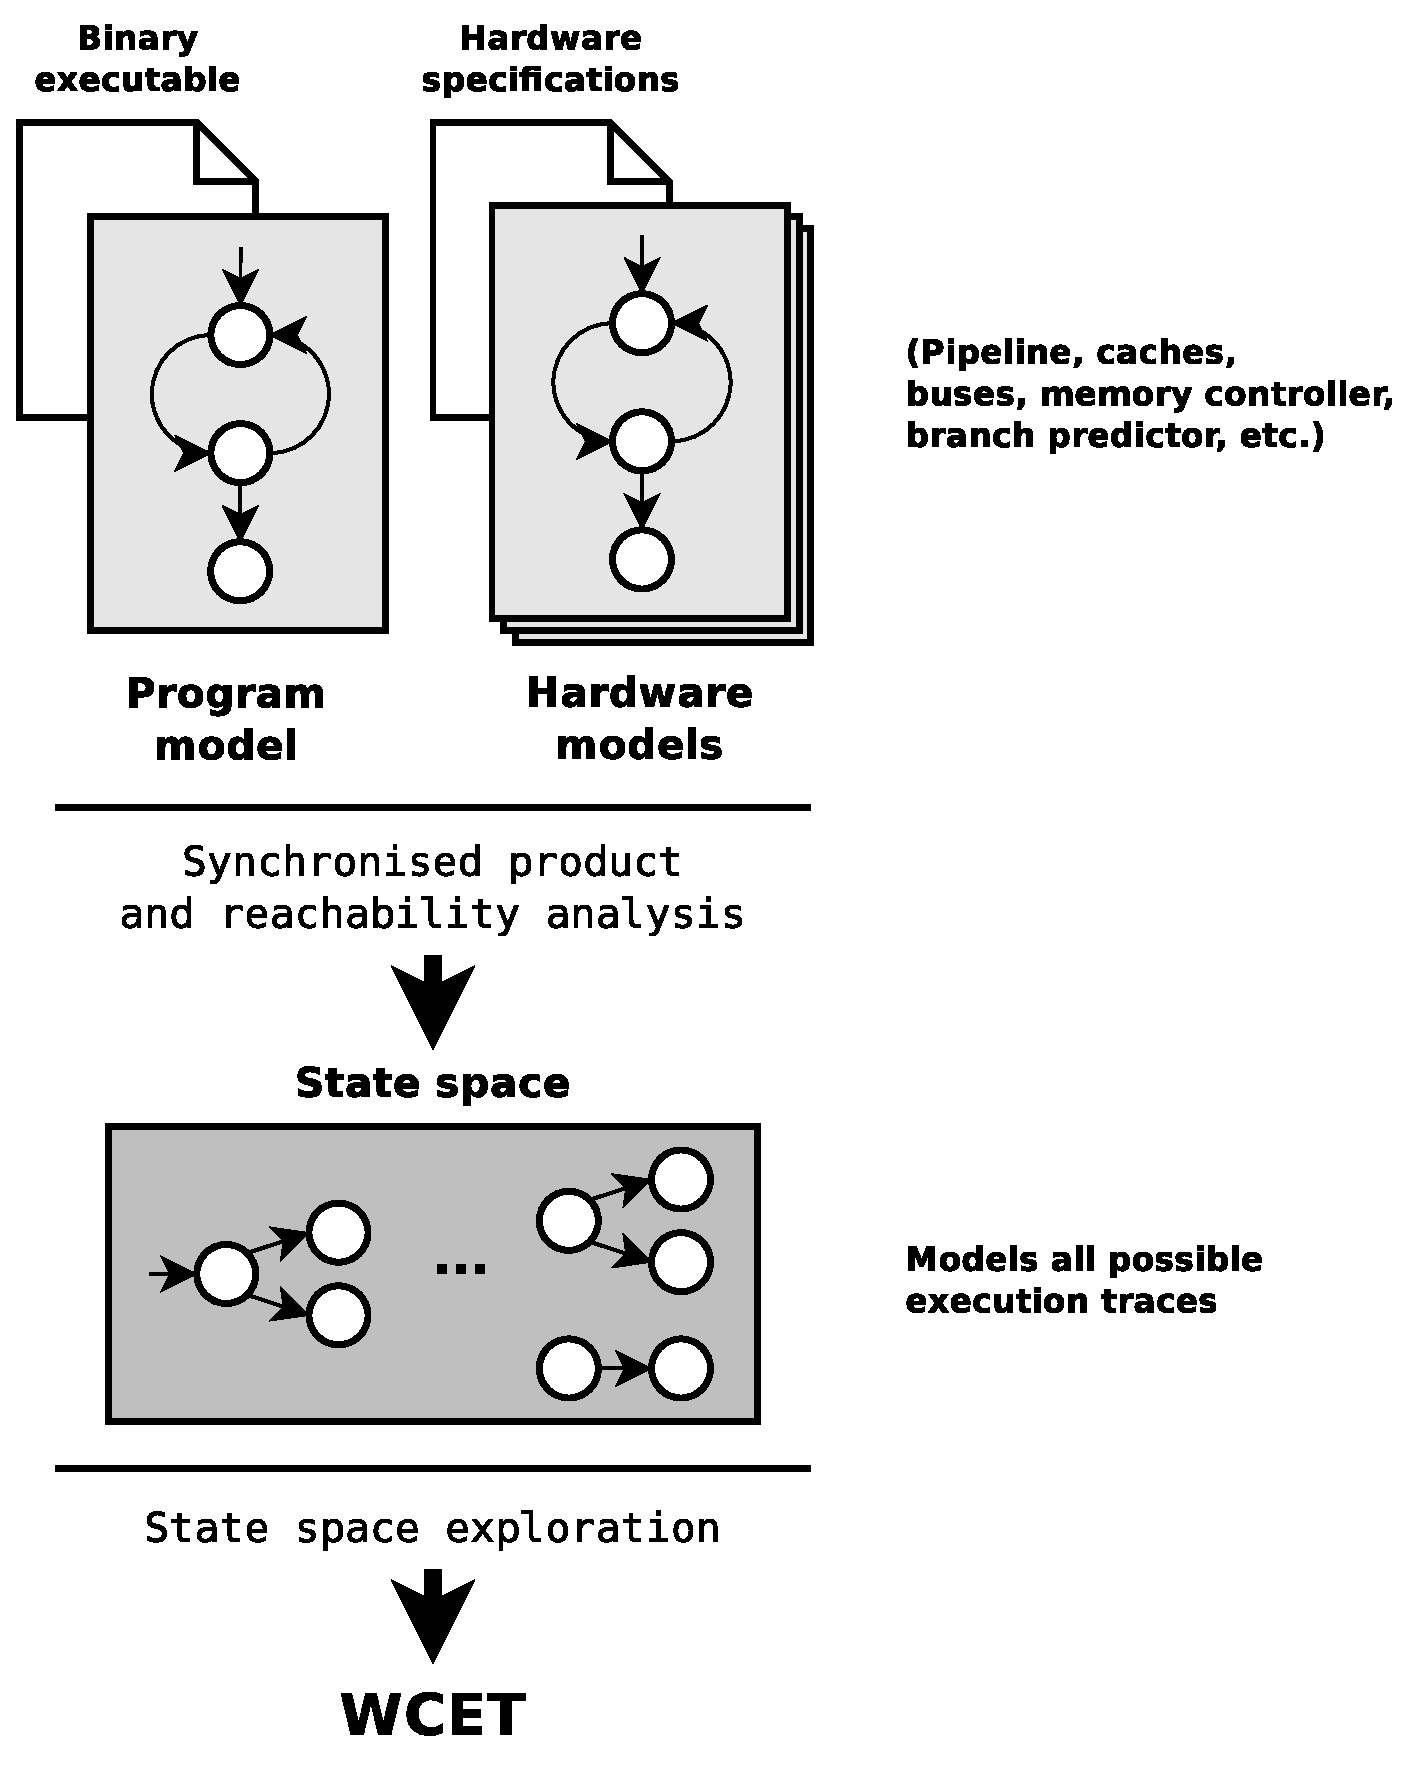
\includegraphics[scale=0.3]{img/model-checking.eps}
    \caption{Principes de l'analyse temporelle par vérification de modèles}
    \label{fig:model-checking}
  \end{figure}

  Différentes approches d'analyse temporelle se basent sur la vérification de
  modèles temporisés. Elles consistent en la vérification du produit synchronisé
  du modèle du programme et du modèle de la plateforme materielle -- cf. figure
  \ref{fig:model-checking}. L'analyse temporelle est alors réduit à un problème
  d'accessibilité temporisée. Ce problème est solvable grâce aux méthodes de
  vérification de modèles temporisés existantes.

  Il existe différents outils d'analyse temporelle à base de vérification de
  modèle \cite{DOT10, CB13}. Les résultats expérimentaux montrent qu'une prise
  en compte moins abstraite des comportements matériels produit des estimations
  du pire cas de temps d'exécution plus précises. Cependant, ces outils
  n'offrent pas de performances acceptables du fait d'une trop forte expansion
  de leur espaces d'état \cite{Wil04}.

  \vspace{1em}

  % Utilisation d'une bibliothèque d'analyse et de transformation de CFG pour le
  % slicing de CFG.
  % Organisation de l'article.

  L'outil d'analyse statique de fichier binaire détaillé ici est implémenté en
  Haskell grace à Hoopl, une bibliothèque de manipulation de CFG
  \cite{RDP10}. Cette bibliothèque permet de définir simplement des analyses de
  flots de données ainsi que des transformations sur les CFG manipulés. La
  section \ref{sec:reconstruction} détaille le processus de reconstruction de
  CFG et la section \ref{sec:simplification} détaille le processus de
  \textit{simplification} de CFG. La section \ref{sec:related-work} évoque
  différentes méthodes de reconstruction de CFG existantes. Enfin, la section
  \ref{sec:conclusion} présente les perspectives de ce travail.

  \section{Background and related works}
\label{sec:relatedworks}

\subsection{Branch prediction basis}
\label{sec:bpbasis}

In modern processors, pipelines are used to improve the instruction execution rate by executing simultaneously different stages of several instructions at the same time.
Each cycle, one (or more in the case of superscalar processor) instruction is fetched sequentially from the memory and fed into the pipeline.
When a branch instruction is executed, the outcome (whether the branch is taken or not, and what is the actual target) is usually not known in the lower stages of the pipeline.
Thus, bubbles\footnote{A bubble, or pipeline stall, is a delay cycle. When a bubble enters a stage, this stage has no activity during the current cycle.} are inserted in these stages until the address of the next instruction is available. These delays are control hazards and have an impact on the execution time.

Branch prediction is a set of techniques used to minimize the occurrence of this situation.
It consists in trying to predict the outcome of a branch instruction when it gets into the pipeline in order to fetch  the correct following instruction with a high probability.
The simplest form of branch prediction is static branch prediction based on the program code only.
A straightforward prediction algorithm is to predict all branches as always not taken.
If the prediction is correct, no cycle is lost.
If the prediction is incorrect, the lower stages of the pipeline have to be flushed to mimic the insertion of bubbles.
A more efficient algorithm widely used is to predict forward branches (conditional statements) as always not taken and backward branches (loops) as always taken.

Dynamic branch prediction uses runtime information to further improve the prediction accuracy.
There is a wide variety of dynamic branch prediction algorithms that cannot be covered here (see~\cite{Engblom2003} for an overview).
From now on, we will focuses on the algorithm analysed in this paper.
It is based on a set of 2-bit saturating counter as illustrated on figure~\ref{fig:sat_counter}.
From left to right, the four states are usually called: taken (11), weakly taken (10), weakly not taken (01), not taken (00).
A counter is associated with a branch instruction.
It is initialized either statically or after the first execution of the branch.
Then, the state evolves according to the actual outcomes of the execution of the instruction: it is incremented when the branch is taken and decremented otherwise.

\begin{figure}
    \centering
    \begin{adjustbox}{width=\textwidth}
        \begin{tikzpicture}[->,>=stealth',shorten >=1pt,auto,node distance=2.8cm,
    semithick,state/.style=state with output]
  \tikzstyle{every state}=[fill=none,draw=black,text=black]

  \node[state]                                     (WNT) {$01$ \nodepart{lower} nt};
  \node[state]                                     (NT) [right of=WNT] {$00$ \nodepart{lower} nt};
  \node[state]                                     (WT) [left of=WNT] {$10$ \nodepart{lower} t};
  \node[state]                                     (T)  [left of=WT] {$11$ \nodepart{lower} t};

  \path (NT)    edge [bend left]  node {taken} (WNT)
        (NT)    edge [loop right] node {not taken} (NT)
        (WNT)   edge [bend left]  node {not taken} (NT)
        (WNT)   edge [bend left]  node {taken} (WT)
        (WT)    edge [bend left]  node {not taken} (WNT)
        (WT)    edge [bend left]  node {taken} (T)
        (T)     edge [bend left]  node {not taken} (WT)
        (T)    edge [loop left]  node {taken} (T);
\end{tikzpicture}

    \end{adjustbox}
    \caption{State machine of a 2-bit saturating counter. Outputs: \texttt{t} for taken, \texttt{nt} for not taken. The initial state is implementation dependant.}
    \label{fig:sat_counter}
\end{figure}

Each of these counters is usually stored along with the target of the branch instruction in an entry of a small cache memory: the BTB. A BTB entry is commonly retrieved with a combination of index and tag computed from the branch instruction.
When the BTB is full, a replacement policy is applied to free an entry.

\subsection{Analysis of branch prediction techniques}

An important body of work is related to WCET analysis for processor with dynamic branch prediction (see for instance~\cite{Colin2000,Bate2004,Maiza2011,Grund2011625,Puffitsch2016}).
Most of these works focus on the analysis of branch prediction (whether a branch is taken or not) but except for~\cite{Colin2000} and~\cite{Grund2011625}, do not take into account branch target prediction (whether the target of the branch is in the BTB or not).
Only~\cite{Grund2011625} analyzes the interactions between the BTB and the instruction prefetch buffer which is mandatory to take into account fine grain penalty for misprediction.
When this interaction is not analyzed, a uniform penalty must be used to account for misprediction, and the hypothesis of the timing compositionality of the architecture must be implicitly assumed (\textsl{i.e.} the analysis can safely follow local worst case path only~\cite{Wilhelm2009}).  
Lastly none of these works tackle the problem of analyzing the interactions between the ICache and the branch prediction mechanism.
Our approach integrates in a single analysis the ICache, the BTB, and the pipeline using an instruction prefetch buffer. 

\subsection{Model checking and WCET analysis of processors}

There is a limited body of work on model checking techniques for the WCET analysis of processors~\cite{Metzner2004,Gustavsson2010,Dalsgaard2010,Cassez2013}.
In~\cite{Dalsgaard2010} and~\cite{Cassez2013}, it is shown that UPPAAL, a state-of-the-art symbolic model checker for (networks of) timed automata, can be used to model and analyze real-life processors.
The target processor of these works feature instruction and data caches and an in-order 5-stage pipeline without dynamic branch prediction.
Our target processor features an ICache and an in-order 5-stage pipeline with a BTB and an instruction prefetch buffer.
Our ICache model is original, but close to the model used in~\cite{Cassez2013}.
Our pipeline model is fully original, as it integrates an instruction prefetch buffer and interactions with an original BTB model.

Following~\cite{Cassez2013}, to improve scalability, our analysis framework uses program slicing to narrow the set of instructions and memory locations that must be accurately modeled in order to compute a sound bound.
%Contrary to~\cite{Cassez2013}, we do not integrate program slicing and construction of the CFG in a single processing step. % Pas nécessaire.
To improve modularity, we use a standalone, state-of-the-art, program slicer for binary code~\cite{wcet16_mangean}.

  %!TEX root = ./main.tex
\section{WCET estimation using model-checking}
\label{sec:modelchecking}

  WCET estimation can be reduced to a reachability problem in a network of timed
  automata~\cite{CB13}. The \textsc{Uppaal} tool that supports timed automata
  extended with bounded integer variables is used to build the models, and to
  solve the reachability problem.

  A model of the hardware is built where each architectural feature
  (pipeline(s), cache(s), bus(es), memory, \dots) is modeled by one or more
  timed automata. These automata are synchronized through {\it channels} to
  model the actual hardware behavior. For instance the automaton modeling the
  fetch stage of a pipeline is synchronized with the automaton modeling the
  instruction cache which is synchronized with the automaton modeling the bus
  and so on. The timings of the hardware are modeled by guards and clocks on
  some edges of the automata. A simple model of a memory controller could be the
  timed automaton of Figure~\ref{fig:memaccess}. Notice that this model accounts
  only for the timing.

  \begin{figure}[b]
    \raggedleft
    \floatbox[{\capbeside\thisfloatsetup{capbesideposition={right,center},capbesidewidth=9.3cm}}]{figure}[\FBwidth]
    {\caption{Simple modeling of a memory using \textsc{Uppaal}. In
        the initial state (on the top left) the memory waits for an
        access (MainMemStart synchronization channel). When the access
        is requested, clock $t$ resets and the automaton remains in
        the bottom right state until $t$ reaches the {\scriptsize
          MAINMEMTRANS} value. Then the memory returns to the initial
        state and notifies the end of the memory access (MainMemEnd
        synchronization channel).}\label{fig:memaccess}}
    {\includegraphics[scale=.6]{fig/automainmem.pdf}}
  \end{figure}

  A model of the program is automatically built from the binary code. In this
  model, each location corresponds to an instruction. An edge leaving a location
  corresponds to the execution of the instruction. For conditional branches, two
  edges leave the location according to the behavior of the branch (taken or not
  taken). Each edge is synchronized with the automaton that models the
  instruction fetch so that it may only be fired if the hardware fetches a new
  instruction. Memory locations are updated according to the semantics of the
  instruction and to its advance in the pipeline. The model of the program has
  an initial state, $I$, that corresponds to the entry point of the program and
  a final state, $F$, that corresponds to the point at which the WCET has to be
  computed.

  At last, a global clock $x$ is used to measure the time. It is initialized at
  0.

  The WCET is then the largest value, $max(x)$, of $x$ when $F$ is
  reached. $max(x)$ can be computed with a model-checker and the following
  reachability property $R(T)$: ``Is $F$ reachable with $x \geq T$ ?''. If
  $R(T)$ is true and $R(T+1)$ is false then $T$ is the WCET of the program.

  This approach is modular since the hardware and software models are built
  separately and the hardware model does not depend on the software to check. No
  assumption is made about the structure of the binary code generated by the
  compiler and the model of the program is built automatically without need for
  annotations

  \paragraph*{Modeling the values stored in memory}

  Data stored in memory and registers -- called a {\it location} in the
  remaining of the paper -- and used by the program can be either included in or
  abstracted away from the model.  Each location included in the model is
  associated with a bounded variable.  When the program accesses a location, the
  timing is computed by the models of the hardware.  If the location is included
  in the model, the associated variable is also read / written.  If the location
  is abstracted away, the data to be written is discarded and any read access
  returns the special value $\bot$.

  On the one hand, every location included in the model adds a dimension to the
  state of the system and thus contributes to the growth of the state space.  On
  the other hand, $\bot$ values can lead the model checker to explore paths that
  are not in the systems when they impact a conditional branch instruction.
  Thus the problem is to automatically compute the minimal set of locations that
  impact on the control flow of the program and that should be included in the
  model.  In this paper, we focus on this problem.


  % !TEX root =  main.tex
\section{Program Slicing}
\label{sec:slicing}

  \subsection{Notations}
  \label{subsec:slicing-notations}

  Let $\mathcal{I}$ be a finite set of instructions. Let $\mathcal{L}$ be a
  totally ordered finite set of labels. A program $P$ is a finite subset of
  $\mathcal{L} \times \mathcal{I}$ such as $\forall (l,i) \in P,\quad (l,i') \in
  P \leftrightarrow i = i'$. We denote $\mathcal{V}$ the set of variables of
  $P$. If we consider the program in Figure~\ref{fig:dump}, $\mathcal{I}$ is the
  subset of instructions of the 32 bits PowerPC instruction set used by the
  program, $\mathcal{L}$ is the set of memory addresses aligned on 4 bytes
  boundaries in the range $[3000, 3034]$ and $\mathcal{V}$ is the set of memory
  locations explicitly or implicitly used (i.e. $\{r1, r3, r8, r9, r10, lr,
  ctr\}$).

  A basic block is a sequence of instructions of $P$ with one entry point, its
  first instruction, and one exit point, its last instruction. A basic block is
  maximal if it is not contained in any other basic block. Let $G_P$ = $\langle
  V_P, E_P, u_{G_P}, v_{G_P} \rangle$ where $V_P$ is the finite set of maximal
  basic blocks of $P$ and $E_P \subset V_P \times V_P$ is such that there is an
  edge between $v_1 \in V_P$ and $v_2 \in V_P$ if and only if the first
  instruction of $v_2$ can be executed immediately after the last instruction of
  $v_1$ in $P$. $u_{G_P} \in V_P$ and $v_{G_P} \in V_P$ are respectively the
  entry block and the exit block of $P$. Then $G_P$ is the CFG of $P$.

  \subsection{General overview}
  \label{subsec:slicing-overview}

  Program slicing has been introduced by Weiser~\cite{Wei81}. Weiser defines
  a program slice as an executable program that is obtained from the original
  program by deleting zero or more statements, computing the same values for a
  given subset of variables of the program. He claims that a slice corresponds
  to the mental abstractions that people make when they are debugging a
  program. The original formulation of program slicing proposed by Weiser is
  based on iterative solutions of data-flow equations. Ottenstein and
  Ottenstein~\cite{OO84} were the first to redefine slicing as a reachability
  problem in a dependence graph representation of a program. They use a Program
  Dependence Graph (PDG)~\cite{FOW87} for static slicing of single-procedure
  structured programs. Efforts have been made to extend this approach to
  unstructured programs~\cite{Agr94,KJL03} and multiple-procedure
  programs~\cite{HSR90,KJL03}. More details on the topic can be found on the
  survey by Tip~\cite{Tip95}.
  
  We consider in this section a toy example to highlight the slicing method. It
  is a simple program that computes iteratively the first 30 values of the
  Fibonacci sequence ($F_{n}=F_{n-1}+F_{n-2}$, with $F_{0}=1$ and $F_{1}=1$).
  The code targets the PowerPC instruction set. The program works as follow:
  \begin{itemize}
    \item The \texttt{\_start} label (Figure~\ref{fig:dump}, line 1) is the
      program entry point. It gets minimal startup code that initializes the
      stack pointer $r1$ and calls the \texttt{main} at $3010$
      (Figure~\ref{fig:dump}, line 7). If the \texttt{main()} function returns,
      it enters in an infinite loop (Figure~\ref{fig:dump}, line 5) ;
    \item Figure~\ref{fig:dump}, lines 8 to 11 initialize the sequence. The loop
      is controlled by the dedicated $ctr$ counter register ;
    \item Figure~\ref{fig:dump}, lines 13 to 16 are the instructions in the
      loop. $r9$ and $r10$ stores respectively the current and the last value
      and are used to compute the next value (in $r3$).
  \end{itemize}
  
  A slice is computed with regards to a slice criterion $\mathcal{C} = \langle
  l, v \rangle$ with $l \in \mathcal{L}$ a label and $v \subseteq \mathcal{V}$ a
  set of variables. So, if we consider the program in Figure~\ref{fig:dump} and
  the slicing criterion $\langle 3030, \{ctr\} \rangle$, i.e. the value of
  register $ctr$ when the instruction pointer contains the address $3030$, we
  obtain the slice shown in Figure~\ref{fig:slice}. Indeed, the instruction
  \verb|bdnz 3024| at address $3030$ (Figure~\ref{fig:slice}, line 16)
  implicitly modifies the register $ctr$, $ctr$ is set by \verb|mtctr r8| at
  $3018$ (Figure~\ref{fig:slice}, line 10) and $r8$ is set by \verb|li r8,29| at
  $3010$ (Figure~\ref{fig:slice}, line 8).
  
  \begin{figure}[ht]
    \centering\scriptsize
    %\hspace{.3cm}
    \subfloat[dump of \texttt{fibcall-O2.elf}]{
      \lstinputlisting[numbers=left, numberstyle=\tiny, frame=single, tabsize=4,
        linewidth=0.8 \linewidth, basicstyle=\linespread{0.5}\ttfamily,
        backgroundcolor=\color{white}]{fig/fibcall-O2.elf.asm}
      \label{fig:dump}}
    \hfill
    \subfloat[slice of \texttt{fibcall-O2.elf} for $\mathcal{C} = \langle 3030, \{ ctr \} \rangle$]{
      \lstinputlisting[numbers=left, numberstyle=\tiny, frame=single, tabsize=4,
        linewidth=0.8 \linewidth, basicstyle=\linespread{0.5}\ttfamily,
        backgroundcolor=\color{white}]{fig/fibcall-O2.elf-slice.asm} 
      \label{fig:slice}}
    \caption{Dump and slice of a binary executable}
  \end{figure}
  
  To compute a slice in binary code, we need to handle arbitrary control flows
  (as opposed to control flow of structured programs) and inter-procedurality.
  In our use case, we must also exclude the techniques that change the order of
  the instructions.  Given all these constraints, we have to use slicing
  techniques based on graph manipulations~\cite{KJL03}.

  This approach is based on the computation of several graphs. The first one is
  the CFG of the program. Figure~\ref{fig:cfg} gives the CFG of
  \verb|fibcall-O2.elf|. Then the Data Dependence Graph (DDG) and the Control
  Dependence Graph (CDG) are computed from the CFG. The DDG captures data
  dependencies between instructions. Its nodes are the instructions of $P$.
  There exists an edge between two nodes of the DDG when the source node does a
  reaching definition of a memory location used by the target node. The CDG
  captures control dependencies between basic blocks. Its nodes are the maximal
  basic blocks of $P$. There exists an edge between two nodes of the CDG when
  the source node determines whether the target node is executed or not.

  After the DDG and the CDG, the next graph is the Program Dependence Graph
  (PDG)~\cite{FOW87}. It is built by merging the DDG and the CDG. Node
  sets of the DDG and the CDG being disjoint (nodes are instructions in the DDG and
  maximal basic blocks in the CDG), the PDG gets its consistency from special
  edges that represent the belonging of a set of instructions to a basic block. In
  summary, the PDG captures the belonging of set of instructions to basic
  blocks, data dependencies at instruction level and control dependencies at
  basic block level. Figure~\ref{fig:pdg} gives the PDG of
  \verb|fibcall-O2.elf|.

  If $P$ does not contain procedure calls, or if these calls are ``inlined''
  when the CFG is built, it is possible to compute slices on the PDG. The slice
  corresponding to a given criterion is obtained by performing a backward
  reachability analysis. The slice is initialized with the slice criterion.
  When an instruction in the slice is the target of a data dependence edge, the
  source instruction is added to the slice. When an instruction in the slice
  belongs to a basic block which is the target of a control dependence edge,
  the last instruction of the source basic block is added to the slice. This
  procedure is iterated until a fixpoint is reached.
  
  \begin{figure}[ht]
    \centering
    \hspace{.5cm}
    \subfloat[CFG of \texttt{fibcall-O2.elf}]{
      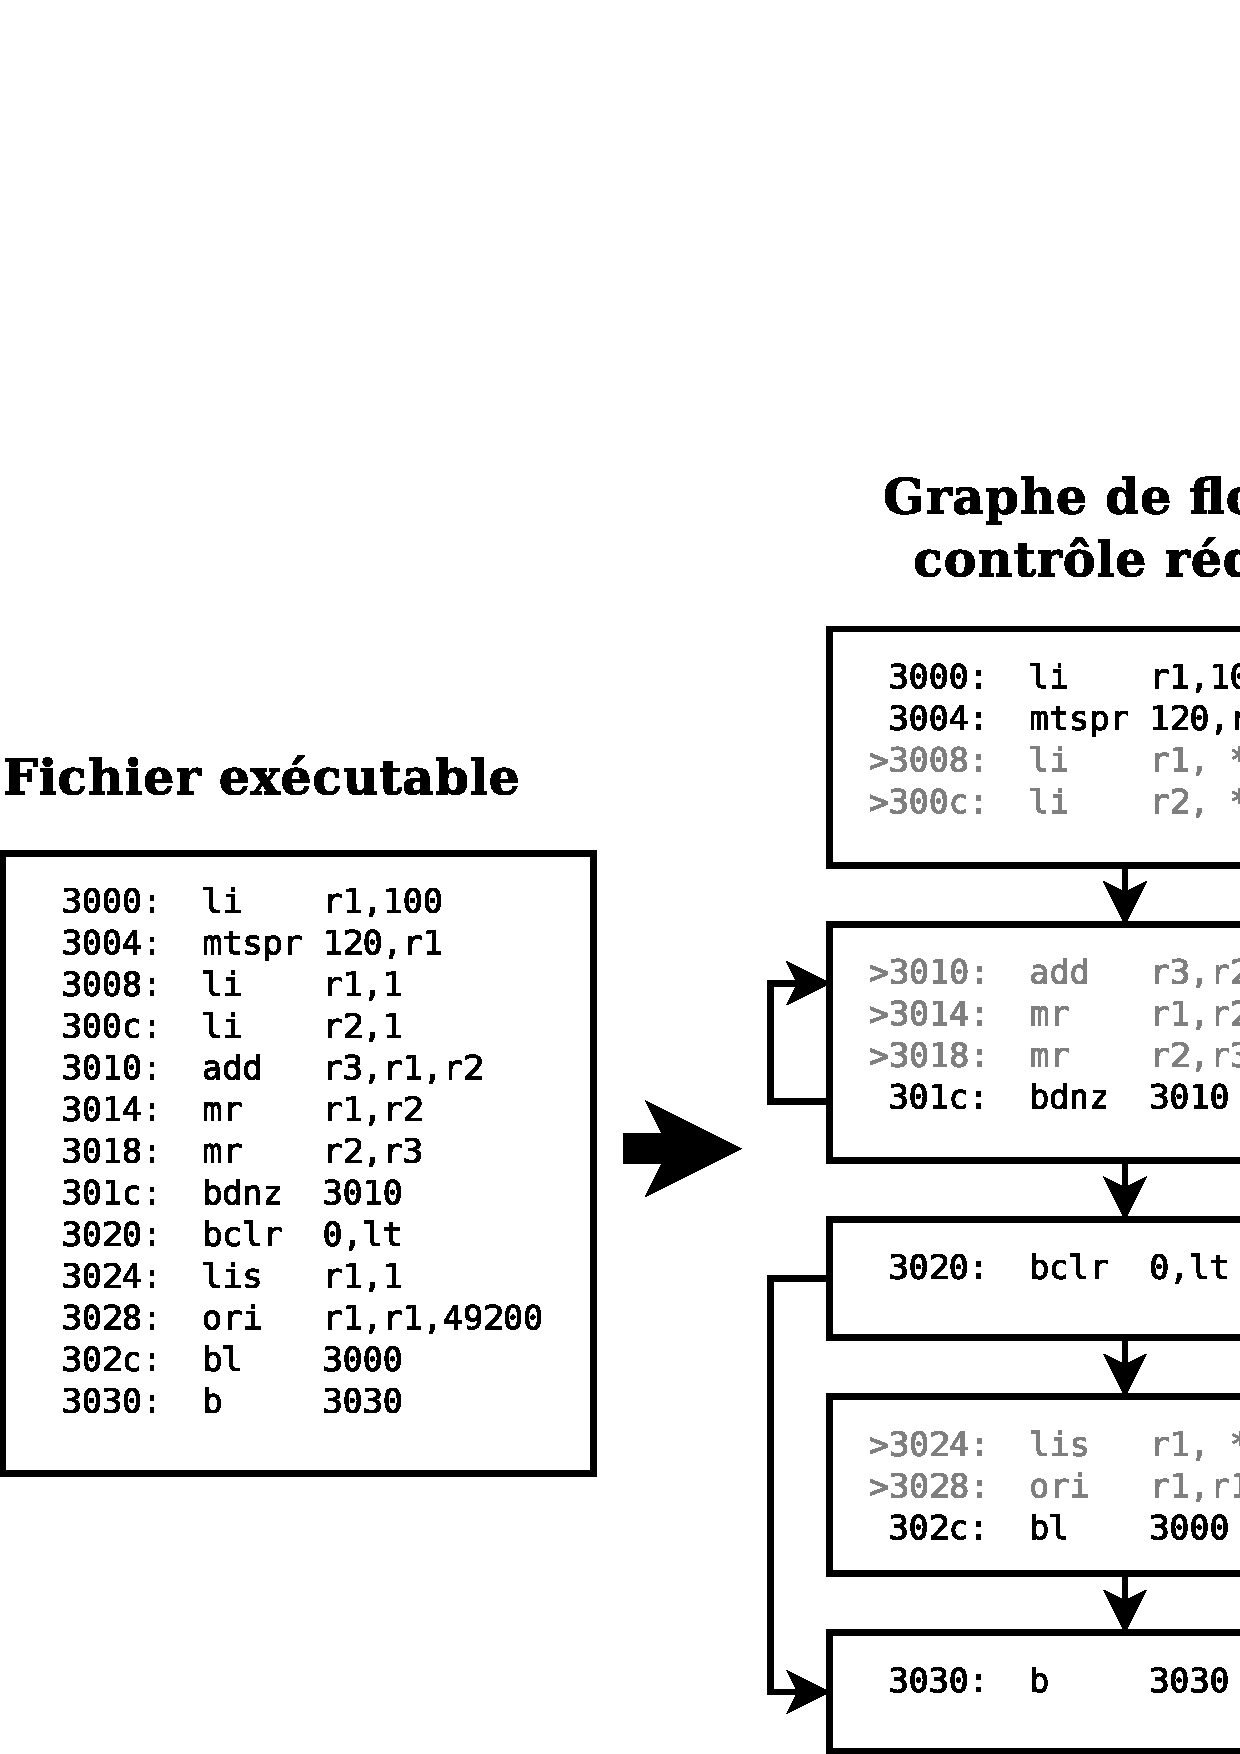
\includegraphics[scale=.4]{fig/cfg.pdf}
      \label{fig:cfg}}
    \hfill
    \subfloat[Simplified PDG of \texttt{fibcall-O2.elf}]{
      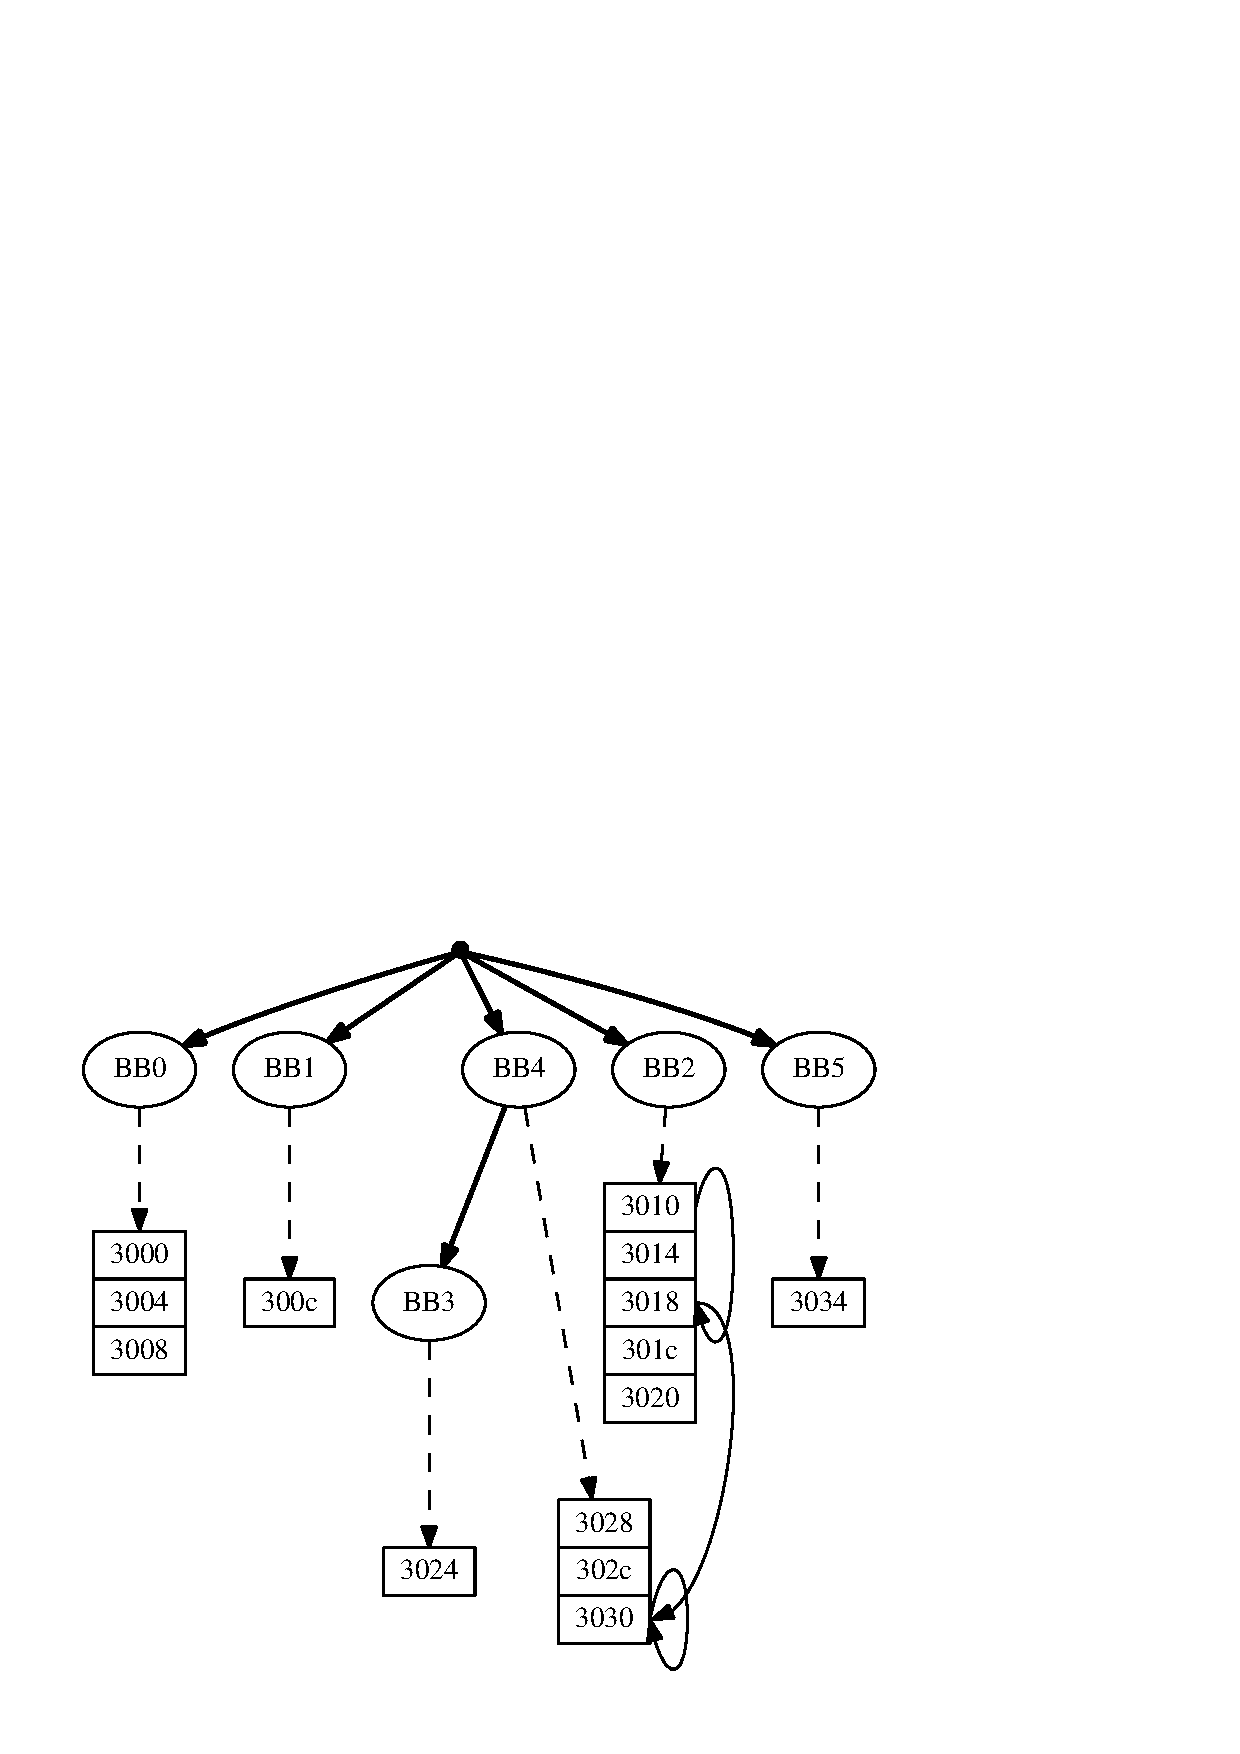
\includegraphics[scale=.4]{fig/pdg.pdf}
      \label{fig:pdg}}    \hspace{.5cm}

    \caption{CFG and PDG of a binary executable}
  \end{figure}

  In Figure~\ref{fig:pdg}, dashed, bold and solid edges represent respectively
  the belonging of a set of instructions to a block, a control dependency
  between two basic blocks, and a data dependency between two instructions.
  Considering once again the program in Figure~\ref{fig:dump} and the slicing
  criterion $\langle 3030, \{ctr\} \rangle$, we obtain the slice shown in
  Figure~\ref{fig:slice}. Indeed, the backward reachability analysis shows that
  the instruction at address $3030$ has a data dependency with the instruction
  at $3018$ which has also a data dependency with the instruction at $3010$ and
  the basic block $BB2$ has no control dependency apart from the entry point.

  Slicing the PDG is suboptimal for programs with procedure calls~\cite{KJL03}.
  %Moreover, inlining functions in the CFG does not scale.
  To overcome this limitation, inter-procedural slicing techniques use a
  fourth graph, the System Dependence Graph (SDG)~\cite{HSR90}. To build the
  SDG, in a first step, the PDG of each procedure must be built. In a second
  step, these PDGs are connected with call, parameter-in and parameter-out edges
  to account for procedure calls and parameters passing. The slicing algorithm
  on the SDG is based on two backwards analyses similar to the one used for the
  PDG. The first backward analysis does not follow parameters-out edges. It only
  adds to the slice instructions up to the entry point. The second backward
  analysis does not follow call and parameter-in edges. It adds to the slice all
  instructions down to the procedures output parameters. As a result, unwanted
  dependencies to output parameters from called procedures are not added to the
  slice.

  \subsection{Abstraction of programs for WCET estimation.}
  \label{subsec:slicing-reduction}
  
  Program slicing has many use cases in software engineering.
  In this paper we
  want to compute the set of memory locations that impact the WCET of a
  program. 
  To determine this set of locations we have to determine a suitable
  slicing criterion. This criterion is the set of pairs $\langle l,v\rangle$
  such that $l$ is the label of a conditional branch instruction and $v$ is the
  set of memory locations read by this instruction. If we consider the program
  in Figure~\ref{fig:dump}, it has only one conditional branch instruction:
  \verb|bdnz 3024| at address $3030$. The branch is taken if the count register
  $ctr$ is not zero. So, to compute the locations that should be part of the
  state of the model we have to compute the slice for the criteria $\{\langle
  3030, \{ctr\} \rangle\}$. The set of variables used either explicitly or
  implicitly by the initial program is $\{r1, r3, r8, r9, r10, lr, ctr\}$. The
  subset of variables used in the slice is $\{r8, ctr\}$ (see
  Figure~\ref{fig:slice}). Only these two registers have to be included in the
  state of the model.

  Let us underline that computing this slice gives us extra informations. For
  each register in the slice, we also know which instructions impact its value
  at a given execution point. In the general case, not all the instructions
  using a register in the slice are in the slice. Such instructions must be
  processed as instructions using registers not in the slice. Their output must
  not be written to the state. This allows to further reduce the number of
  states to explore.
  

  \section{Implémentation}
\label{sec:implementation}
  
  % Utilisation d'un analyseur sémantique de fichiers exécutables pour la
  % reconstruction de CFG.

  Notre outil manipule des fichiers binaires exécutables compilés pour des
  cibles embarquées à base de microprocesseurs PowerPC. Les informations
  nécessaires à la classification des instructions utiles à la reconstruction
  d'un CFG et au \emph{program slicing} sont issues d'une analyse syntaxique et
  sémantique du fichier binaire exécutable. Cette analyse est produite par un
  outil généré par HARMLESS \cite{KBB12}, un générateur de simulateurs basé sur
  un langage de description de plateformes matérielles.

  \begin{figure}[ht]
    \centering
    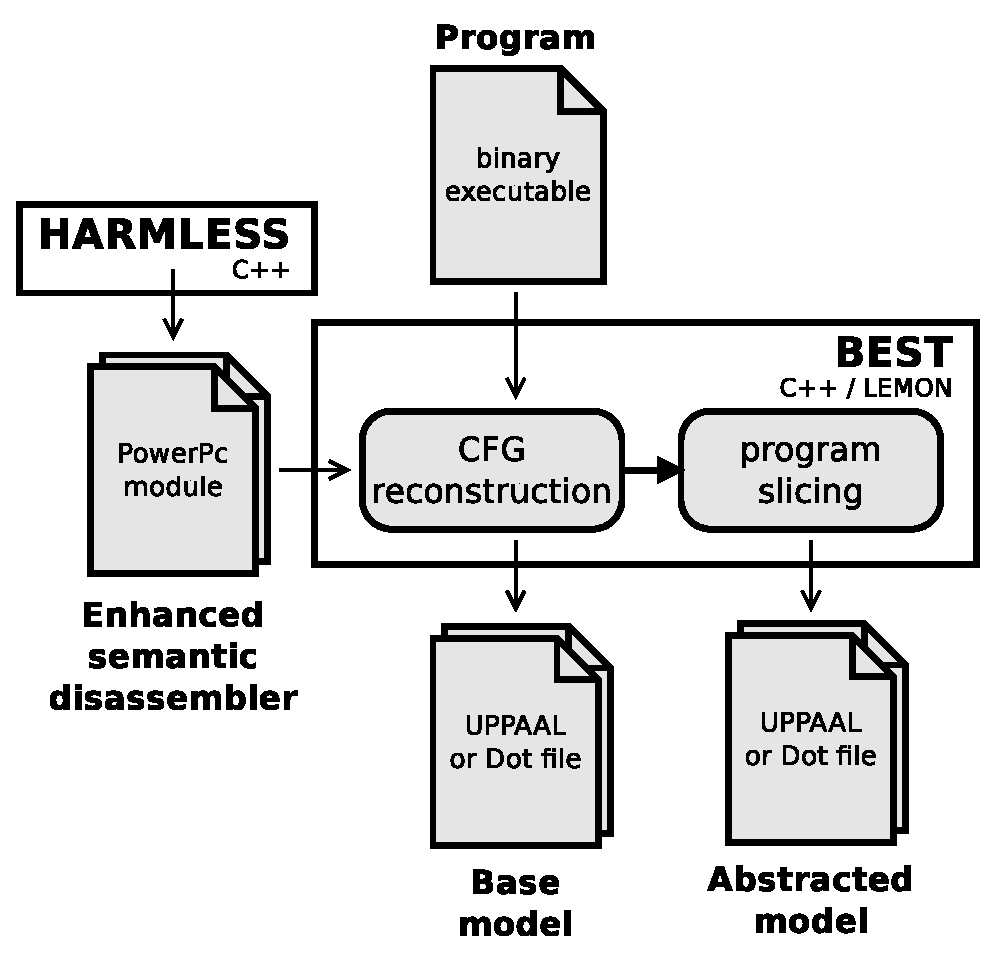
\includegraphics[scale=0.5]{img/archi.eps}
    \caption{Structuration de l'outil}
    \label{fig:implem}
  \end{figure}

  %% Utilisation de la propagation de constante pour rafiner le CFG.
    
  %% Afin de permettre la déterminaison de certaines cibles de saut il est une
  %% nouvelle fois fait usage de l'outil HARMLESS. Celui-ci réalise une
  %% simulation de l'exécution de notre programme sur la plateforme matérielle
  %% considérée. Il est donc possible de procéder à une propagation de constantes
  %% permettant de déterminer des plages de valeurs pour certains registres.

  Notre outil est développé en langage C++, il s'appuie sur une bibliothèque de
  gestion de graphe : LEMON \cite{DJK11}. Les modèles du programme obtenus avant
  ou après \emph{slicing} peuvent être exporter au format Dot, pour être
  visualisés, ainsi que sous forme d'automates temporisés \cite{AD94} au format
  UPPAAL \cite{LPY97}.
  
  Différents tests ont été réalisés à partir des \emph{benchmarks} de Mälardalen
  \cite{GBA10}. Ces \emph{benchmarks} sont utilisés pour évaluer et comparer
  différents outils et méthodes de calcul de pire cas de temps d'exécution.

  \begin{tabular}{ |l| |c|c|c|c| |c|c| }
    \hline
      \multirow{2}{*}{Source file}
    & \multicolumn{4}{c||}{\textsc{Gcc}}
    & \multicolumn{2}{c|}{\textsc{Cosmic}}
      
  \\\cline{2-7}
    & \emph{default} & \verb|-O1|     & \verb|-O2| & \verb|-O3|
    & \verb|-no|     & \emph{default}

  \\\hline
      \verb|adpcm.c|
    & -32\% (19) & -12\% (34) & -7\% (30) & -8\% (38)
    & -38\% (39) & -38\% (39)

  \\\hline
      \verb|bs.c|
    & -31\% (13) & -23\% (13) & -10\% (10) & -10\% (10)  
    & -29\% (14) & -15\% (13)

  \\\hline
      \verb|bsort100.c|
    & -21\% (14) & -25\% (20) & -31\% (16) & -31\% (16)
    & -13\% (15) & -13\% (15)
      
  \\\hline
      \verb|cnt.c|
    & -29\% (17) & -25\% (20) & -38\% (16) & -40\% (20)  
    & -69\% (39) & -69\% (39) 

  \\\hline
      \verb|compress.c|
    & -19\% (21) & -15\% (33) & -9\% (35) & -8\% (37)  
    & -41\% (39) & -41\% (39) 

  \\\hline
      \verb|crc.c|
    & -47\% (19) & -36\% (25) & -52\% (21) & -57\% (21)
    & -49\% (39) & -49\% (39) 

  \\\hline
      \verb|expint.c|
    & -33\% (15) & -36\% (28) & -64\% (11) & -64\% (11)  
    & -59\% (39) & -59\% (39) 

  \\\hline
      \verb|fdct.c|
    & -47\% (15) & -83\% (23) & -88\% (32) & -91\% (35)
    & -92\% (37) & -92\% (37)

  \\\hline
      \verb|fibcall.c|
    & -31\% (13) & -42\% (12) & -57\% (7) & -57\% (7) 
    & -50\% (12) & -40\% (10) 

  \\\hline
      \verb|fir.c|
    & -50\% (18) & -38\% (24) & -30\% (23) & -30\% (23)
    & -56\% (39) & -56\% (39) 

  \\\hline
      \verb|janne_complex.c|
    & -36\% (14) & -33\% (9) & -25\% (8) & -22\% (9) 
    & -82\% (38) & -13\% (8) 

  \\\hline
      \verb|jfdctint.c|
    & -23\% (13) & -80\% (15) & -85\% (27) & -89\% (35)
    & -92\% (37) & -92\% (37) 
      
  \\\hline
      \verb|matmult.c|
    & -43\% (21) & -23\% (22) & -19\% (21) & -29\% (21)
    & -74\% (39) & -74\% (39) 
      
  \\\hline
      \verb|ndes.c|
    & -42\% (19) & -21\% (29) & -11\% (28) & -3\% (30)  
    & -54\% (39) & -56\% (39) 
      
  \\\hline
      \verb|ns.c|
    & -31\% (16) & -24\% (17) & -13\% (15) & -25\% (12)  
    & -59\% (39) & -58\% (38) 
      
  \\\hline
      \verb|prime.c|
    & -20\% (15) & -33\% (9) & -33\% (9) & -25\% (8)   
    & -66\% (38) & -63\% (38) 
      
  \\\hline
\end{tabular}

  \section{Conclusion}
\label{sec:conclusion}

%Using model checking for WCET analysis has been debated.
In this paper we show that model checking can be used to analyze the complex interactions between the components of a microarchitecture used in safety critical embedded control systems.
We focus on the interaction between the instruction cache, the branch prediction unit, and a pipeline with an instruction buffer.
Model checking provides a solution to perform an integrated analysis of the whole system.
This integrated analysis allows to explore only feasible traces of the system and to compute the actual sequence of memory access requests and pipeline stall states corresponding to each trace.
Our result are promising concerning the scalability of the approach for such systems.

In future works, we shall extend our analysis framework to support programs
that use the stack to store data that impact the control flow. We also want to
produce results using more complex benchmarks, and explore the impact of non-determinism concerning the initial state of the micro-architecture (eg. cache and BTB state).
We will also tend toward having a model aligned with the actual e200z4 core (\textsl{i.e.} adding a second way to the pipeline) in order to validate our model against a real system through microbenchmarks.
Our long term objective is to model and analyze a multiprocessor architecture based on e200z4 core such as the MPC5643L.


  
  \appendix
  \bibliographystyle{plain}
  \bibliography{src/refs}

\end{document}
